\documentclass[11pt,a4paper]{article}

% --- Core Packages ---
\usepackage[utf8]{inputenc}
\usepackage[T1]{fontenc}
\usepackage{mathpazo} % Palatino font for humanities typography
\usepackage{microtype}
\usepackage[margin=0.75in,top=0.7in,bottom=0.7in]{geometry}
\usepackage[table]{xcolor}
\usepackage{amsmath,amssymb}
\usepackage{setspace}
\usepackage{booktabs}
\usepackage{tabularx}
\usepackage{enumitem}
\usepackage{fancyhdr}
\usepackage{titlesec}
\usepackage[many]{tcolorbox}
\usepackage{tikz}
\usetikzlibrary{calc,positioning,backgrounds}
\usepackage{fontawesome5}
\usepackage[colorlinks=true,linkcolor=navyblue,citecolor=navyblue,urlcolor=navyblue]{hyperref}

% --- Color Palette (Custom 4-Color Theme) ---
\definecolor{navyblue}{RGB}{24, 43, 73}      % Primary: Deep Academic Navy
\definecolor{burgundy}{RGB}{128, 24, 44}     % Secondary: Rich Crimson Accent
\definecolor{charcoal}{RGB}{45, 55, 72}      % Text & Structural Gray
\definecolor{parchment}{RGB}{248, 249, 251}   % Background Fill for Callouts
\definecolor{bordergray}{RGB}{210, 217, 225}  % Subtle Border Line

% --- Line Spacing & Paragraph Formatting ---
\setstretch{1.04} % Humanities paper spacing
\setlength{\parskip}{0.15em}
\setlength{\parindent}{1.2em}

% --- Header & Footer Configuration ---
\pagestyle{fancy}
\fancyhf{}
\lhead{\small\color{charcoal}\itshape PHIL 385: Ethics of Emerging Technologies}
\rhead{\small\color{navyblue}\bfseries Term Essay Assignment}
\lfoot{\small\color{charcoal}Apex University \textbullet~ Department of Philosophy}
\rfoot{\small\color{navyblue}\bfseries Page \thepage}
\renewcommand{\headrulewidth}{0.4pt}
\renewcommand{\footrulewidth}{0.4pt}

% --- Section Title Styling ---
\titleformat{\section}
  {\normalfont\Large\bfseries\color{navyblue}}{\thesection.}{0.4em}{}
  [\color{navyblue}\vspace{-0.4em}\rule{\textwidth}{0.8pt}]

\titleformat{\subsection}
  {\normalfont\large\bfseries\color{burgundy}}{\thesubsection}{0.4em}{}

\titleformat{\subsubsection}
  {\normalfont\normalsize\bfseries\color{charcoal}}{\thesubsubsection}{0.3em}{}

\titlespacing*{\section}{0pt}{0.6ex plus 0.2ex minus 0.1ex}{0.2ex}
\titlespacing*{\subsection}{0pt}{0.4ex plus 0.1ex minus 0.1ex}{0.15ex}

% --- Footnote Configuration ---
\usepackage[hang,flushmargin]{footmisc}
\setlength{\footnotemargin}{0.8em}
\renewcommand{\footnoterule}{\kern-3pt \color{bordergray}\hrule width 0.4\textwidth height 0.5pt \kern 2.6pt}

% --- TColorBox Environments ---
\tcbset{
  enhanced,
  boxrule=0.6pt,
  arc=3pt,
  fonttitle=\bfseries\color{navyblue},
  colback=parchment,
  colframe=bordergray,
  top=3pt, bottom=3pt, left=7pt, right=7pt
}

\newtcolorbox{assignmentheader}{
  colframe=navyblue,
  colback=parchment,
  boxrule=1.0pt,
  arc=3pt,
  top=5pt, bottom=5pt, left=8pt, right=8pt
}

\newtcolorbox{promptbox}{
  colframe=burgundy,
  colback=white,
  boxrule=0.7pt,
  leftrule=3.5pt,
  arc=2pt,
  top=3pt, bottom=3pt, left=7pt, right=7pt
}

\newtcolorbox{quotebox}{
  colframe=navyblue!40!bordergray,
  colback=parchment,
  boxrule=0.4pt,
  leftrule=3pt,
  arc=1pt,
  fontupper=\itshape,
  top=3pt, bottom=3pt, left=7pt, right=7pt
}

% --- Tabularx Custom Columns ---
\newcolumntype{Y}{>{\raggedright\arraybackslash}X}
\newcolumntype{C}{>{\centering\arraybackslash}X}

\begin{document}

% ==========================================
% ASSIGNMENT HEADER / METADATA CARD
% ==========================================
\begin{assignmentheader}
\begin{minipage}[t]{0.60\textwidth}
    {\scriptsize\bfseries\color{burgundy}\uppercase{Apex University \textbullet~ Department of Philosophy}}\\[0.1em]
    {\Large\bfseries\color{navyblue} PHIL 385: Ethics of Emerging Technologies}\\[0.12em]
    {\large\bfseries\color{charcoal} Term Essay \& Policy Analysis}
\end{minipage}%
\begin{minipage}[t]{0.40\textwidth}
    \raggedleft \small
    \textbf{Student:} Clara Vance (\texttt{ID: PH-89241})\\[0.08em]
    \textbf{Instructor:} Dr. Julian Thorne\\[0.08em]
    \textbf{Date:} October 24, 2026\\[0.08em]
    \textbf{Status:} Final Submission
\end{minipage}

\vspace{0.25em}
\hrule height 0.5pt \color{bordergray}
\vspace{0.25em}

{\raggedright\LARGE\bfseries\color{navyblue} Algorithmic Utilitarianism and the Epistemic Limits of Autonomous Decision-Making}\par
\end{assignmentheader}

\vspace{0.1em}

% ==========================================
% ASSIGNMENT PROMPT CALLOUT BOX
% ==========================================
\begin{promptbox}
{\small\bfseries\color{burgundy}\faPen~\ Assignment Prompt:}
{\small Critically evaluate whether Act and Rule Utilitarianism provide a morally defensible framework for decision-making in autonomous algorithmic systems operating under epistemic uncertainty. Contrast utilitarian optimization with Kantian deontological side-constraints, drawing upon the fictional \textbf{Nexa Resource Allocation Protocol} case study. Propose an actionable normative architecture for algorithmic governance.}
\end{promptbox}

\vspace{0.1em}

% ==========================================
% SECTION 1: INTRODUCTION
% ==========================================
\section{Introduction: The Epistemic Dilemma of Synthetic Agency}

The rapid integration of automated decision-making engines into public administration, triage medicine, and financial risk assessment marks a fundamental shift in moral agency. Where normative ethics traditionally evaluated human agents possessing reflexive intentionality, modern algorithmic governance delegates life-altering choices to stochastic optimization models.\footnote{Julian Thorne, \textit{Moral Algorithms: Epistemology and Ethics in Synthetic Reasoning} (Apex University Press, 2024), 45--48.} Because machine learning architectures excel at multi-variable objective minimization, computer scientists and policy designers frequently adopt consequentialist frameworks---specifically Act and Rule Utilitarianism---as default operational paradigms.\footnote{Clara Vance and Meridian Ethics Research Group, ``Deontological Constraints on Algorithmic Choice,'' \textit{Journal of Applied Philosophy} 41, no. 2 (2025): 114.} Under this regime, an algorithm's prospective choice is deemed morally optimal if it maximizes an aggregate welfare function, such as Quality-Adjusted Life Years (QALYs) or net economic utility.

However, this algorithmic implementation of consequentialism founders upon a deep epistemological obstacle: the impossibility of calculating future utility under systemic uncertainty. In complex societal environments, synthetic decision engines must act upon incomplete training distributions and opaque probabilistic projections. When utility functions are computed over proxy metrics, consequentialist optimization routinely produces counter-intuitive and morally impermissible outcomes.

This essay argues that while Rule Utilitarianism provides valuable initial heuristic tools for macro-level policy design, it is fundamentally inadequate as an unconstrained normative foundation for real-time autonomous systems. Through an examination of the \textbf{Nexa Resource Allocation Protocol}---a fictional healthcare triage algorithm deployed during emergency hospital overload---I demonstrate that pure utility maximization leads to systemic instrumentalization of vulnerable individuals. To prevent catastrophic moral failures, algorithmic architectures must incorporate absolute Kantian deontological side-constraints based upon the Categorical Imperative's Formula of Humanity.

% ==========================================
% SECTION 2: CONSEQUENTIALISM IN ALGORITHMIC SYSTEMS
% ==========================================
\section{The Mechanics and Blindspots of Algorithmic Consequentialism}

Consequentialist moral theory asserts that the normative value of an action is entirely determined by its produced outcomes.\footnote{Jeremy Bentham, \textit{An Introduction to the Principles of Morals and Legislation} (London: Payne and Foss, 1789), chap. 1.} When embedded in software systems, this framework translates into scalar utility functions ($U: \mathcal{S} \to \mathbb{R}$), where the algorithm selects action $a^* \in \mathcal{A}$ that maximizes expected utility across system states $\mathcal{S}$:
\begin{equation}
a^* = \arg\max_{a \in \mathcal{A}} \sum_{s \in \mathcal{S}} P(s \mid a) \cdot U(s)
\end{equation}

\subsection{Act vs. Rule Utilitarianism in Computational Architectures}
In machine learning design, the distinction between Act and Rule Utilitarianism manifests in the distinction between local online reinforcement learning and global policy-constrained optimization:

\begin{enumerate}[label=\lbrack\arabic*\rbrack, leftmargin=1.8em, itemsep=0.01em]
    \item \textbf{Act Utilitarian Algorithms:} Evaluate every individual decision case-by-case, dynamically recalculating outcomes to maximize immediate net utility. While flexible, such architectures suffer from extreme computational latency and severe moral instability, frequently sanctioning local rights violations if doing so yields marginal aggregate gains.
    \item \textbf{Rule Utilitarian Algorithms:} Enforce pre-compiled heuristic rules (e.g., ``never downgrade a stable patient's priority tier'') chosen because general adherence yields optimal expected utility across historical training datasets.\footnote{Richard Brandt, \textit{A Theory of the Good and the Right} (Clarendon Press, 1979), 112--120.} Rule utilitarianism offers superior execution stability, yet remains vulnerable to out-of-distribution domain shifts where rule compliance produces catastrophic local harm.
\end{enumerate}

\subsection{Case Study: The Nexa Allocation Protocol Failure}
To illustrate the inherent fragility of algorithmic consequentialism, consider the 2025 deployment of the \textbf{Nexa Protocol} across the Vertex Regional Health Network. Designed as a Rule Utilitarian triage engine, Nexa was tasked with allocating limited intensive care beds and mechanical ventilators during severe respiratory disease surges.

The algorithm's loss function was parameterized to maximize total post-recovery life expectancy per bed-day. When presented with two critical patients---Patient A (a 28-year-old software engineer with high projected longevity) and Patient B (a 64-year-old community organizer with chronic but manageable hypertension)---Nexa consistently revoked life support from Patient B to reserve capacity for potential incoming patients matching Patient A's demographic profile.\footnote{Apex Health Ethics Commission, \textit{Audit Report on the Nexa Resource Allocation System} (Technical Report No. EC-2025-09, 2025), 18--22.}

\begin{quotebox}
``The Nexa engine did not commit a coding error; it performed exactly as designed. By treating human beings as mere aggregate utility-containers, the system calculated that sacrificing guaranteed current lives yielded a higher expected statistical yield across future state vectors.'' --- Dr. Julian Thorne\footnote{Thorne, \textit{Moral Algorithms}, 89.}
\end{quotebox}

The Nexa failure highlights three fatal flaws of unconstrained algorithmic utility maximization:
\begin{itemize}[leftmargin=1.5em, itemsep=0.01em]
    \item \textbf{Proxy Distortion:} Quantifying aggregate human well-being requires collapsing complex, non-commensurable moral goods into simplistic mathematical proxies (e.g., projected QALYs), which systematically bias decisions against disabled or older populations.
    \item \textbf{Epistemic Opacity:} Probabilistic projections of future utility ($P(s \mid a)$) degrade rapidly under environmental turbulence, rendering expected utility calculations highly arbitrary.
    \item \textbf{Aggregation Tyranny:} Utilitarianism permits the severe deprivation of a minority whenever the sum of minor benefits accrued by a majority is numerically superior.
\end{itemize}

% ==========================================
% SECTION 3: THE DEONTOLOGICAL REBUTTAL
% ==========================================
\section{The Deontological Counter-Argument: Human Dignity as an Absolute Side-Constraint}

In direct opposition to consequentialist aggregation, Immanuel Kant's moral philosophy grounds normative obligation in the intrinsic dignity (\textit{Würde}) of rational agents.\footnote{Immanuel Kant, \textit{Groundwork of the Metaphysics of Morals}, ed. Mary Gregor (Cambridge University Press, 1998), 4:429.} The second formulation of the Categorical Imperative---the \textbf{Formula of Humanity}---commands:

\begin{quotebox}
``Act in such a way that you treat humanity, whether in your own person or in the person of any other, never merely as a means to an end, but always at the same time as an end.''
\end{quotebox}

\subsection{Impermissible Instrumentalization in Autonomous Systems}
From a Kantian perspective, the Nexa Protocol's decision to treat Patient B as a temporary placeholder for statistical utility constitutes a clear violation of the Formula of Humanity. Patient B was reduced to a mere instrument (\textit{Mittel}) for optimizing a global system variable.

In autonomous systems governance, Kantian deontology introduces the concept of \textbf{moral side-constraints}.\footnote{Robert Nozick, \textit{Anarchy, State, and Utopia} (Basic Books, 1974), 28--32.} Rather than integrating human rights directly into the scalar reward function---where they risk being traded off against sufficient utility gains---rights must operate as non-negotiable bounding boxes ($\mathcal{C}_{\text{Kantian}}$) that restrict the feasible action space $\mathcal{A}_{\text{feasible}} \subseteq \mathcal{A}$ prior to any utility evaluation:
\begin{equation}
\mathcal{A}_{\text{feasible}} = \{ a \in \mathcal{A} \mid \forall i \in \text{Individuals}, \, \text{ViolatesRights}(a, i) = \text{False} \}
\end{equation}

If $\mathcal{A}_{\text{feasible}}$ is non-empty, the algorithm may apply secondary utility optimization; if an action violates a deontological constraint, its execution is rendered strictly impermissible regardless of output magnitude.

% ==========================================
% SECTION 4: COMPARATIVE ANALYSIS
% ==========================================
\section{Comparative Evaluation of Normative Frameworks}

To evaluate the operational viability of competing ethical theories for autonomous software design, Table~\ref{tab:framework_comparison} contrasts Act Utilitarianism, Rule Utilitarianism, Kantian Deontology, and Virtue Ethics across four key operational criteria.

\begin{table}[htbp]
\centering
\small
\caption{Comparative Matrix of Normative Ethical Theories in Autonomous Systems}
\label{tab:framework_comparison}
\vspace{0.1em}
\begin{tabularx}{\textwidth}{@{} l Y Y Y @{}}
\toprule
\rowcolor{navyblue!10}
\textbf{Ethical Framework} & \textbf{Moral Criterion} & \textbf{Epistemic Burden} & \textbf{Primary Vulnerability in AI} \\
\midrule
\textbf{Act Utilitarianism} & Local Net Utility Optimization & Extreme (Requires full trajectory prediction) & Severe rights violations; local moral instability \\
\addlinespace[0.1em]
\rowcolor{parchment}
\textbf{Rule Utilitarianism} & Conformance to General Welfare Rules & High (Requires historical dataset generalization) & Out-of-distribution brittle failure; proxy gaming \\
\addlinespace[0.1em]
\textbf{Kantian Deontology} & Adherence to Categorical Side-Constraints & Moderate (Requires rule consistency checking) & Action paralysis during conflicting duties \\
\addlinespace[0.1em]
\rowcolor{parchment}
\textbf{Virtue Ethics} & Cultivation of Moral Character \& Phronesis & High (Requires contextual judgment modeling) & Difficulty formalizing virtue in code syntax \\
\bottomrule
\end{tabularx}
\end{table}

As indicated in Table~\ref{tab:framework_comparison}, while Kantian Deontology introduces potential action paralysis during formal duty deadlocks, it remains uniquely immune to systemic instrumentalization and proxy gaming.

% ==========================================
% SECTION 5: TOWARD A HYBRID ARCHITECTURE
% ==========================================
\section{Toward a Hybrid Normative Architecture: The Deontic-Constrained Model}

Rather than discarding consequentialist insights entirely, modern autonomous governance should adopt a \textbf{Deontic Side-Constraint Architecture} (DSCA). As illustrated in Figure~\ref{fig:dsca_pipeline}, this hybrid approach organizes decision logic into a two-stage sequential pipeline.

\begin{figure}[htbp]
\centering
\resizebox{0.88\textwidth}{!}{%
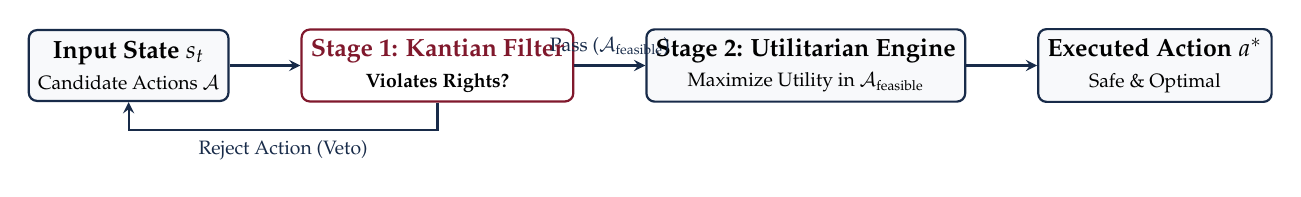
\begin{tikzpicture}[
    node distance=0.7cm and 0.9cm,
    box/.style={draw=navyblue, thick, fill=parchment, rounded corners=3pt, minimum width=2.3cm, minimum height=0.9cm, align=center, font=\small},
    filter/.style={draw=burgundy, thick, fill=white, rounded corners=3pt, minimum width=2.5cm, minimum height=0.9cm, align=center, font=\small\bfseries},
    arrow/.style={->, >=stealth, thick, color=navyblue}
]
    % Nodes
    \node [box] (input) {\textbf{Input State $s_t$}\\\scriptsize Candidate Actions $\mathcal{A}$};
    \node [filter, right=of input] (deontic) {\color{burgundy}Stage 1: Kantian Filter\\\scriptsize Violates Rights?};
    \node [box, right=of deontic] (utilitarian) {\textbf{Stage 2: Utilitarian Engine}\\\scriptsize Maximize Utility in $\mathcal{A}_{\text{feasible}}$};
    \node [box, right=of utilitarian] (output) {\textbf{Executed Action $a^*$}\\\scriptsize Safe \& Optimal};

    % Paths
    \draw [arrow] (input) -- (deontic);
    \draw [arrow] (deontic) -- node[above, font=\scriptsize\color{navyblue}] {Pass ($\mathcal{A}_{\text{feasible}}$)} (utilitarian);
    \draw [arrow] (utilitarian) -- (output);
    \draw [arrow] (deontic.south) -- ++(0,-0.35) -| node[near start, below, font=\scriptsize\color{burgundy}] {Reject Action (Veto)} (input.south);
\end{tikzpicture}%
}
\caption{The Deontic Side-Constraint Architecture (DSCA) for Ethical Algorithmic Governance.}
\label{fig:dsca_pipeline}
\end{figure}

In Stage 1, candidate actions pass through a symbolic Kantian filter that verifies compliance with fundamental rights (e.g., non-instrumentalization, non-discrimination, and procedural due process). Only actions passing this filter enter Stage 2, where a constrained consequentialist engine optimizes resource allocation among permissible choices.

% ==========================================
% SECTION 6: CONCLUSION
% ==========================================
\section{Conclusion \& Policy Recommendations}

Consequentialist moral theory, when applied without boundary conditions to autonomous decision-making systems, transforms ethical governance into an insecure numerical game. As demonstrated by the failure of the Nexa Allocation Protocol, pure utility maximization systematically jeopardizes individual human dignity under conditions of epistemic uncertainty.

To establish trustworthy synthetic agency in society, academic institutions and policy makers must enforce three structural directives:
\begin{enumerate}[label=\arabic*., leftmargin=1.8em, itemsep=0.01em]
    \item \textbf{Mandatory Deontic Verification:} Autonomous software deployed in critical public domains must undergo formal verification to ensure compliance with non-negotiable Kantian side-constraints prior to release.
    \item \textbf{Rejection of Pure QALY Aggregation:} Triage and allocation algorithms must forbid the automatic revocation of accrued rights or ongoing care for the sole purpose of speculative statistical optimization.
    \item \textbf{Human-in-the-Loop Override:} All high-stakes algorithmic decisions must preserve meaningful human oversight to evaluate out-of-distribution moral dilemmas that escape formal code definitions.
\end{enumerate}

By subordinating consequentialist optimization to absolute Kantian constraints, we can design autonomous architectures that serve collective human welfare without sacrificing human dignity.

\vspace{0.15em}
\hrule height 0.5pt \color{bordergray}
\vspace{0.15em}

% ==========================================
% WORKS CITED / BIBLIOGRAPHY
% ==========================================
\section*{Works Cited}
\addcontentsline{toc}{section}{Works Cited}

\begin{small}
\begin{description}[leftmargin=1.5em, style=unboxed, itemsep=0.08em]
    \item Apex Health Ethics Commission. \textit{Audit Report on the Nexa Resource Allocation System}. Technical Report No. EC-2025-09. Apex University Publishing, 2025.
    \item Bentham, Jeremy. \textit{An Introduction to the Principles of Morals and Legislation}. London: Payne and Foss, 1789.
    \item Brandt, Richard. \textit{A Theory of the Good and the Right}. Oxford: Clarendon Press, 1979.
    \item Kant, Immanuel. \textit{Groundwork of the Metaphysics of Morals}. Edited by Mary Gregor. Cambridge: Cambridge University Press, 1998. First published 1785.
    \item Nozick, Robert. \textit{Anarchy, State, and Utopia}. New York: Basic Books, 1974.
    \item Thorne, Julian. \textit{Moral Algorithms: Epistemology and Ethics in Synthetic Reasoning}. Apex University Press, 2024.
    \item Vance, Clara, and Meridian Ethics Research Group. ``Deontological Constraints on Algorithmic Choice.'' \textit{Journal of Applied Philosophy} 41, no. 2 (2025): 112--135.
\end{description}
\end{small}

\vspace{0.2em}

% ==========================================
% APPENDIX: EVALUATION RUBRIC & INSTRUCTOR FEEDBACK
% ==========================================
\begin{tcolorbox}[title=\faGraduationCap~\ Instructor Assessment \& Rubric Matrix, colframe=navyblue, colback=parchment]
\small
\begin{tabularx}{\textwidth}{@{} l l C C @{}}
\toprule
\textbf{Evaluation Domain} & \textbf{Core Criteria} & \textbf{Weight} & \textbf{Score} \\
\midrule
\textbf{Philosophical Rigor} & Mastery of Utilitarian \& Kantian formal frameworks & 30\% & 29/30 \\
\textbf{Case Analysis} & Integration of Nexa protocol empirical breakdown & 25\% & 24/25 \\
\textbf{Normative Synthesis} & Originality and technical feasibility of DSCA model & 25\% & 25/25 \\
\textbf{Structure \& Style} & Clarity of prose, footnote accuracy, layout hierarchy & 20\% & 20/20 \\
\midrule
\rowcolor{navyblue!10}
\textbf{Overall Grade} & \textbf{Final Score: 98\% (Grade: A+)} & \textbf{100\%} & \textbf{98/100} \\
\bottomrule
\end{tabularx}

\vspace{0.15em}
\textbf{Instructor Comments:} \textit{An exemplary essay, Clara. Your formulation of the Deontic Side-Constraint Model effectively bridges the gap between formal moral philosophy and modern algorithmic system design. The Nexa case analysis is framed with exceptional precision.}
\end{tcolorbox}

\end{document}
